%----------------------------------------------------------------------------
\chapter{A poros plazma kísérlet}
%----------------------------------------------------------------------------


{\color{red}
	A poros plazma kísérletek során elektromos gázkisülési
        plazmába szilárd szemcséket (port) szórunk, amelyek
        elektromos töltésre tesznek szert, és az így
        előállított erősen kölcsönható sokrészecske rendszert
        figyeljük meg. Adott alacsony nyomású gáz terében elhelyezett
        elektródákra kapcsolt feszültséggel  
	lehetséges plazmát létrehozni. Az elektromos táplálás lehet
        egyenáramú, vagy váltakozó áramú a rádiófrekvenciás vagy akár
        a mikrohullámú tartományban. A rádiófrekvenciával váltakozó
        villamos tér a töltéssel rendelkező szabad elektronokra 
	olyan erővel hat, hogy azok felgyorsulva, a háttérgáz semleges
        atomjaival ütközve azokat gerjeszteni és ionizálni tudják, így
        hozzájárulva a szabad töltéshordozók szaporításához.
	A leszakadó elektronok a térben szabadon a ráható erőknek
        megfelelően mozognak és továbbí ütközésekben vehetnek részt
        egészen addíg, míg valamely elektródán elnyelődnek.
	Ez makroszkópikus skálán az eredetileg szigetelő gáz vezető
        plazmává válását jelenti.  

A kísérlet során az előbb említett elektromos gázkisülésbe plazma terébe szórt porszemcsék alatt
	$100nm - 20\mu m$ nagyságú részecskéket értünk, melyek anyaga
        lehet például $SiO_2$, $Al_2O_3$ vagy 
	melamin-formaldehid (MF). A porrészecskék a plazmával
        interakcióba lépve negatívan feltöltődnek az azokat érő ion-,
        és elektronáramok eredményeként. A szemcsék töltés per tömege
        aránya sok nagyságrenddel kisebb a háttérplazma atomos összetevőinél,
        aminek hatására a mozgásuk karakterisztikus ideje légyegesen
        hosszabb az ionokénál is. A szemcsék
        mozgását a környezetük időben kiátlagolt hatásai dominálják,
        vagyis dinamikájuk jórészt lecsatolódik az atomos háttérplazma
        gyors változásairól. Ennek következtében, sok esetben a
        töltött porszemcsékből álló rendszert önmagában tekinthetjük
        egy egykomponensű rendszernek, annak tudatában, hogy a
        a szemcsék töltését és az összetartáshoz szükséges
        peremfeltételeket a gázkisülés biztosítja.
}	

	A porrészecskék transzportjának megértéséhez szükséges a ráható erők azonosítása.
	A különféle erők nagysága a porrészecskék nagyságá{\color{red}val} különféleképpen skálázódik. Elhanyagolásokat
	ennek megfelelően tehetünk.
	\begin{description}
		\item[Gravitációs $F_g$ erő:] Mikrogravitációban végzett kísérletek és nanométer nagyságú részecskék esetén
			elhanyagolhatóak, de a jelen esetben használt mikrométer nagyságú részecskék esetén dominánsak,
		\item[Villamos tér keltette $F_e$ erő:] A porrészecske töltésével és a villamos tér nagyságával
			arányos. A megfelelően irányított villamos térrel lehetséges a részecskék levitációja,  
		\item[Háttératomon való szóródás $F_n$:] A porrészecske driftje során a háttératomokkal való
			{\color{red} ütközéseinek} makroszkópikus erőként való számításba vétele,
		\item[Hőmérséklet gradiensi $F_{th}$ erő:] A gáz hőmérsékletének gradiense okozta
			gázatomok diffúzív jellegű mozgása által okozott indirekt erőhatás,
		\item[Ion sodrási $F_i$ erő:] Az ionokra ható villamos tér okozta {\color{red}ionáramok} hatása a
			porrészecskékre.
	\end{description}
	A poros plazma analízise során fontos szerepet játszik a porrészecskék csatolása.
	A csatolást gyengének és erősnek kategorizáljuk aszerint, hogy a részecskék szomszédja általi
	átlagos potenciális energia az átlagos termikus (kinetikus) energiájához képest kissebb vagy
	nagyobb.
	A csatolást a Coulomb csatolási paraméterrel ($\Gamma$) lehet számosítani, ami a szomszédos
	részecskék Coulomb potenciáljának és termikus energiájának {\color{red}hányadosa}:
	\begin{equation}
		\Gamma = \cfrac{1}{4\pi\varepsilon_0}
                \cfrac{Q^2}{ak_{\rm B}T_d} 
	\end{equation}
	ahol $Q$ a részecskék töltése, $a$ az átlagos részecske
        távolság{\color{red}ával arányos Wigner-Seitz sugár (amely a
          szemcsék sűrűségéből számolható $a^2_{\rm 2D}=1/\pi n$,
          illetve $a^3_{\rm 3D}=3/4\pi n$ formulákkal, a rendszer
          dimenzionalitásától függően)} és a $k_{\rm B}T_d$ a por
        {\color{red} komponens egy részecskére jutó átlagos kinetikus energiája}.
	Ha a $\Gamma$ értéke egy kritikus érték fölé {\color{red}kb.} $\Gamma > 150$ növekszik, akkor
	Ikawa jóslata szerint a porrészecskék {\color{red}sokasága}
        kristályszerkezetbe rendeződik \cite{Ikawa} \todo{bibtex req.}.
	
	 {\color{red}Poros plazmák tudatos alkalmazása jelenleg leginkább
           tudományos természetű, bár létezésükre szennyeződésként
           az iparben figyeltek fel először. Ez pl. VLSI áramkörök gyártásakor
           (plazma alapú maratás során) jelentkezik, ahol a kezelt
           felületre visszahulló szemcsék rövidzárlatot és egyéb
           hibákat okozhatnak, ami a kihozatal csökkenéséhez
	vezet. Laboratóriumi környezetben hasznos modellrendszerei
        lehetnek az atomos (hagyományos) anyagokban lejátszódó
        makroszkopikus folyamatok mikroszkopikus részleteinek
        feltárásához \cite{mikro}. \todo{bibtex req.}} 

%----------------------------------------------------------------------------
\section{A kísérlet}
%----------------------------------------------------------------------------
	A kísérlet lebonyolítására egy speciális kamrára van szükség, amiben lehetséges a plazma
	létrehozása, a porrészecskék szórása illetve a megfelelő villamos tér létrehozása.
	A kamrának hermetikusan jól zártnak kell lennie, hogy csak a kívánt gázt tartalmazza.
	A középvákuumú működéshez kétlépéses vákuumszivattyút kell alkalmazni.
	
	
	A kamra sematikus ábrája a \ref{fig:meresch}. ábrán látható.
	A porrészecskék levitációjáért a villamos tér felelős. A síkba való zárás parabolikus
	potenciállal lehetséges. Az ilyen tér létrehozása a következő elektróda elrendezéssel lehetséges:
	alul elhelyezett korong alakú elektróda, ami felett egy gyűrű alakú elektróda helyezkedik el.
	Az ilyen elektródarendszerre kapcsolt váltakozó feszültség a beszórt porrészecskéket lebegtetni
	tudja. Továbbá a részecskék követéséhez azokat lézerrel megvilágítjuk és nagysebességű kamerával
	felvételt készítünk róla.
	
	\begin{figure}[H]
		\centering
		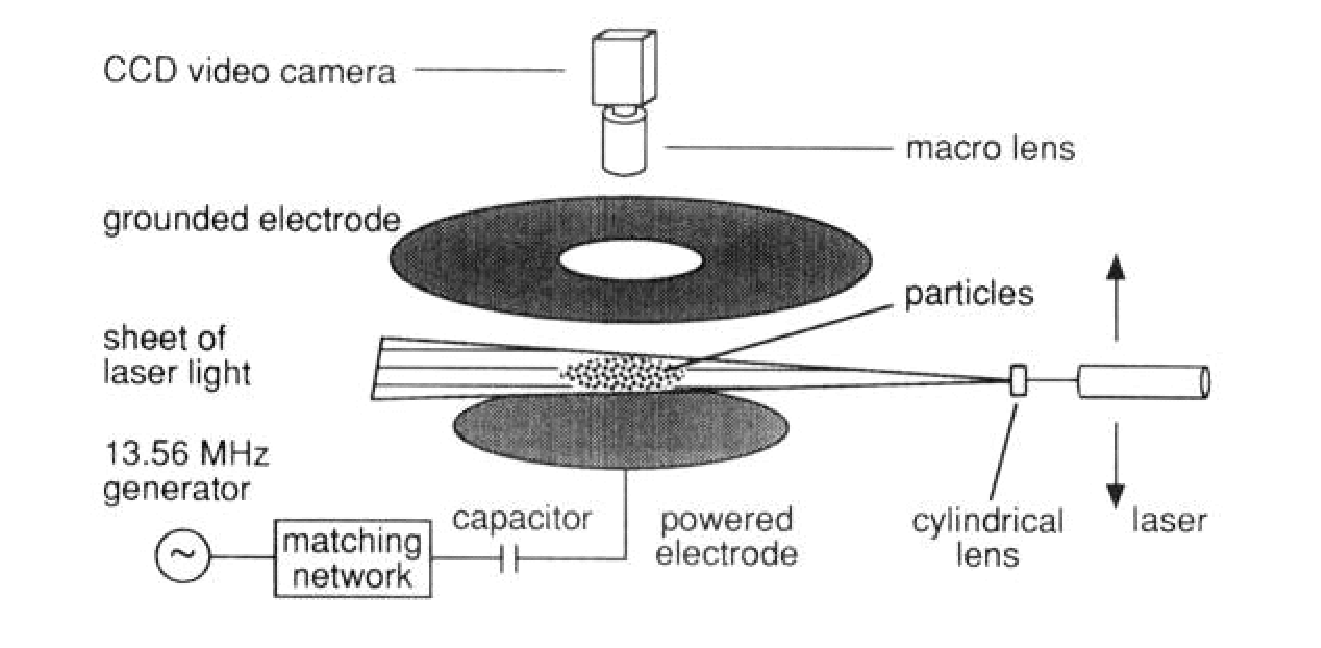
\includegraphics[width=0.9\columnwidth]{figures/eps/dust_camera.eps}
		\caption[A mérési elrendezés sematikus ábrája]{A mérési elrendezés sematikus ábrája (forrás: \cite{Merlino2006})} 
		\label{fig:meresch}
	\end{figure}
	
	A kamrát (\ref{fig:kamra}. ábra) Hartmann Péter külső konzulensem építette és a MTA Wigner FK SZFI
	Gázkisülési Laboratóriumában található.
	
	\noindent A paraméterei:
	\begin{myitemize*}
		\item Kamra belső átmérője: $25$~cm
		\item Kamra belső magassága: $18$~cm
		\item Alsó elektróda átmérője: $18$~cm
		\item Felső gyűrű elektróda belső átmérője: $15$~cm
		\item Felső elektróda távolsága az alsótól: $13$~cm
		\item Argon gáz nyomása: $1.2\pm0.05$~Pa
		\item Gáz átfolyása: $\sim 0.01$~sccm
		\item RF gerjesztés: $7W\ @ \ 13.56$~MHz
		\item Porrészecske: melamin-formaldehid
		\item Porrészecske átmérője: $4.38\pm 0.06~\mu$m
		\item Porrészecske tömege. $6.64\cdot10^{-14} $~kg
		\item Látható porrészecskék száma: $\sim 2500$
		\item Megvilágító lézer: $200~mW$ @  $532~nm$
		\item Kamera: $1.4$~MPixel @ $100$~FPS
	\end{myitemize*}
	{\color{red}Opcionálisan} kamra alsó elektródáját lehetséges egy motorral forgásba
        hozni. Az elektróda felületének érdessége által a kamrában
	lévő gáz is forgásba jön. A gáz forgása az $F_n$ sodrási erővel hat a porrészecsékre.
	{\color{red}A forgó rendszerrel együttforgó viszonyítási
          rendszerben fellépő Coriolis tehetetlenségi erő extrém nagy
          mágneses tér Lorentz erejével ekvivalens hatást gyakorol a
          porszemcsékre, megkerülve ezzel a valódi mágnesek
          alkalmazásával együttjáró nehézségeket.}
	\begin{figure}[H]
		\centering
		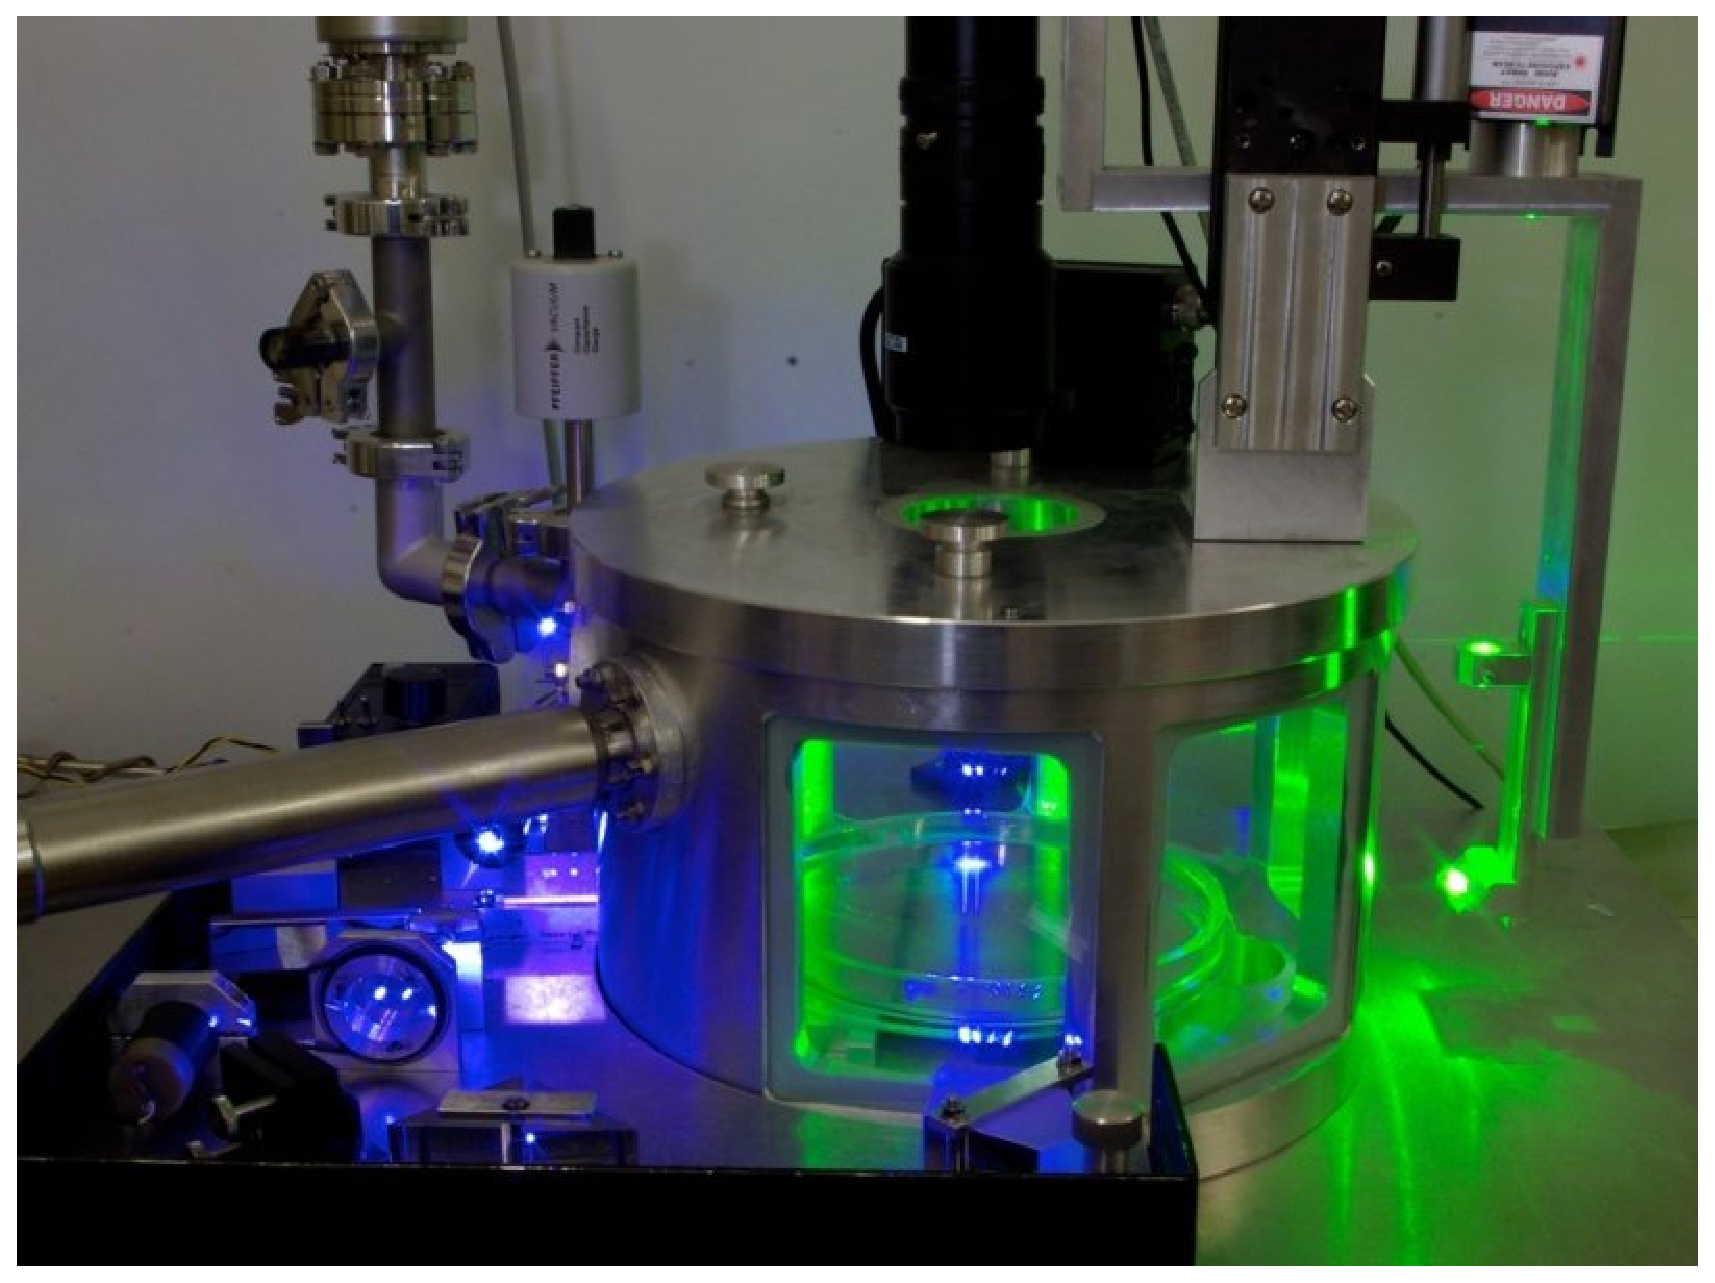
\includegraphics[width=0.9\columnwidth]{figures/eps/dusty2.eps}
		\caption{A konkrét kamra működése közben} 
		\label{fig:kamra}
	\end{figure}



%----------------------------------------------------------------------------
\section{Használt kamera tulajdonságai}
%----------------------------------------------------------------------------
\todo{lehet h az OPENCL után kéne}
%\usepackage{graphics} is needed for \includegraphics
\begin{figure}[!h]
\begin{center}
  \includegraphics[width=0.75\columnwidth,page=2]{Prosilica_GX_DataSheet_1050_en.pdf}
  \caption[A kamera adatlapja]{A kamera adatlapja (forrás: \cite{gx1050})}
  \label{fig:cam_doc}
\end{center}
\end{figure}

%\usepackage{graphics} is needed for \includegraphics
\begin{figure}[htp]
\centering
	\subfloat[A használt kamera.]{
		\includegraphics[width=0.95\columnwidth]{figures/camera.jpg}%
		\label{fig:cam_pic}
	}
	\\
	\subfloat[A kamera beállításainak és a képének megjelenítésére alkalmas tool.]{
		\missingfigure{VimbaViewer kamera szoftver}
		\label{fig:cam_sw}
	}
	\caption[A használt kamera és a hozzá biztosított SW.]{A használt kamera és a hozzá biztosított SW.
	(forrás \cite{gx1050})}
	\label{fig:cam}
\end{figure}

\clearpage

	
%----------------------------------------------------------------------------
\section{A mérendő mennyiségek és a származtatott értékek}
%----------------------------------------------------------------------------
	A kísérlet előkészítése a következő lépésekből áll:
	\begin{enumerate*}
		\item Elővákuum {\color{red}(rotációs)} szivattyú bekapcsolása,
		\item Középvákuum {\color{red}(turbómolekuláris)} szivattyú bekapcsolása,
		\item Argon palack megnyitása a megfelelő áramlás szintjére,
		\item RF gerjesztés bekapcsolása,
		\item Megvilágító lézer bekapcsolása,
		\item \label{it:por} Porrészecskék beszórása,
		\item Kamera bekapcsolása és a megjelenítő szoftver futtatása,
		\item Ha sok összetapadt porrészecske látható, illetve ha túl sok porrészecske látható, akkor
		az RF gerjesztés gyors ki-be kapcsolása után a \ref{it:por}.-től való folytatása a folyamatnak.
	\end{enumerate*}
	A \ref{fig:captures}. ábrán látható álló és forgó alsó elektródájú kísérlet során a
	porrészecskékről készült kép.
	
	\begin{figure}[!ht]
		\centering
		\subfloat[Álló elektróda esetén sok $\left(\sim 1500\right)$ részecske]{
			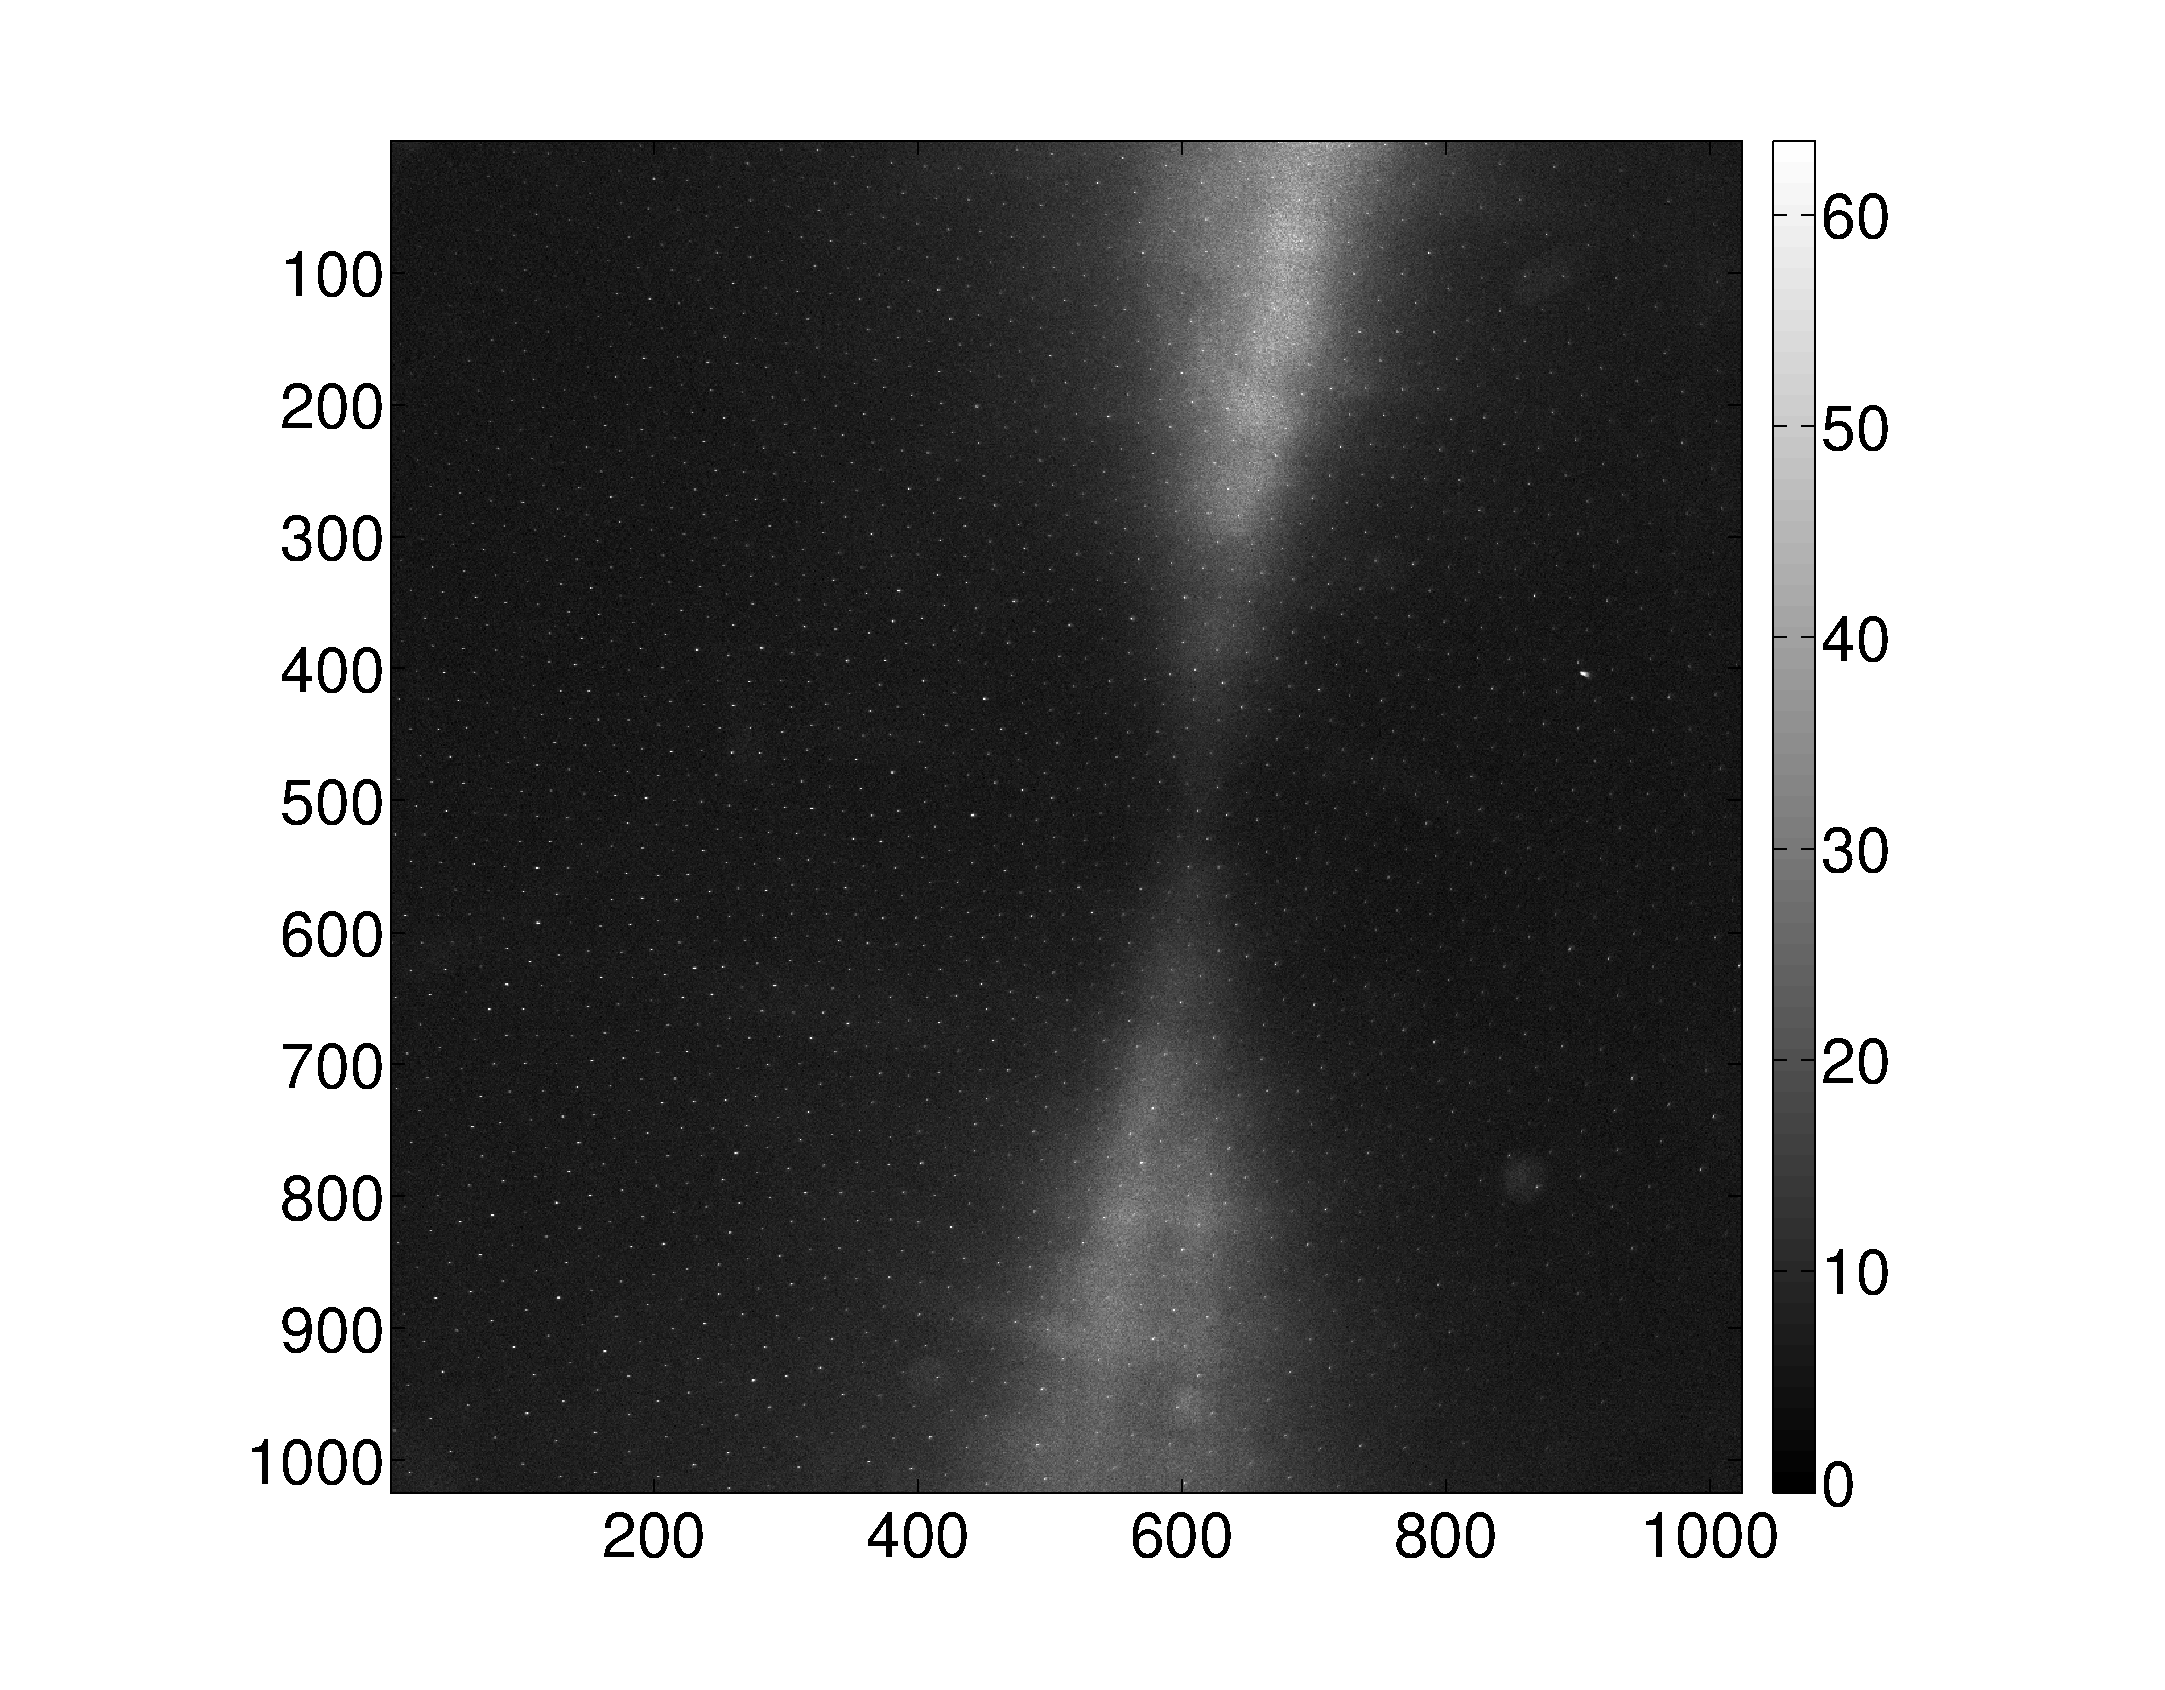
\includegraphics[width=0.95\columnwidth]{figures/eps/000047659380.eps}%
			\label{fig:allo}
		}
		\\
		\subfloat[Forgó elektróda esetén kevés $\left(\sim 100\right)$ részecske]{
			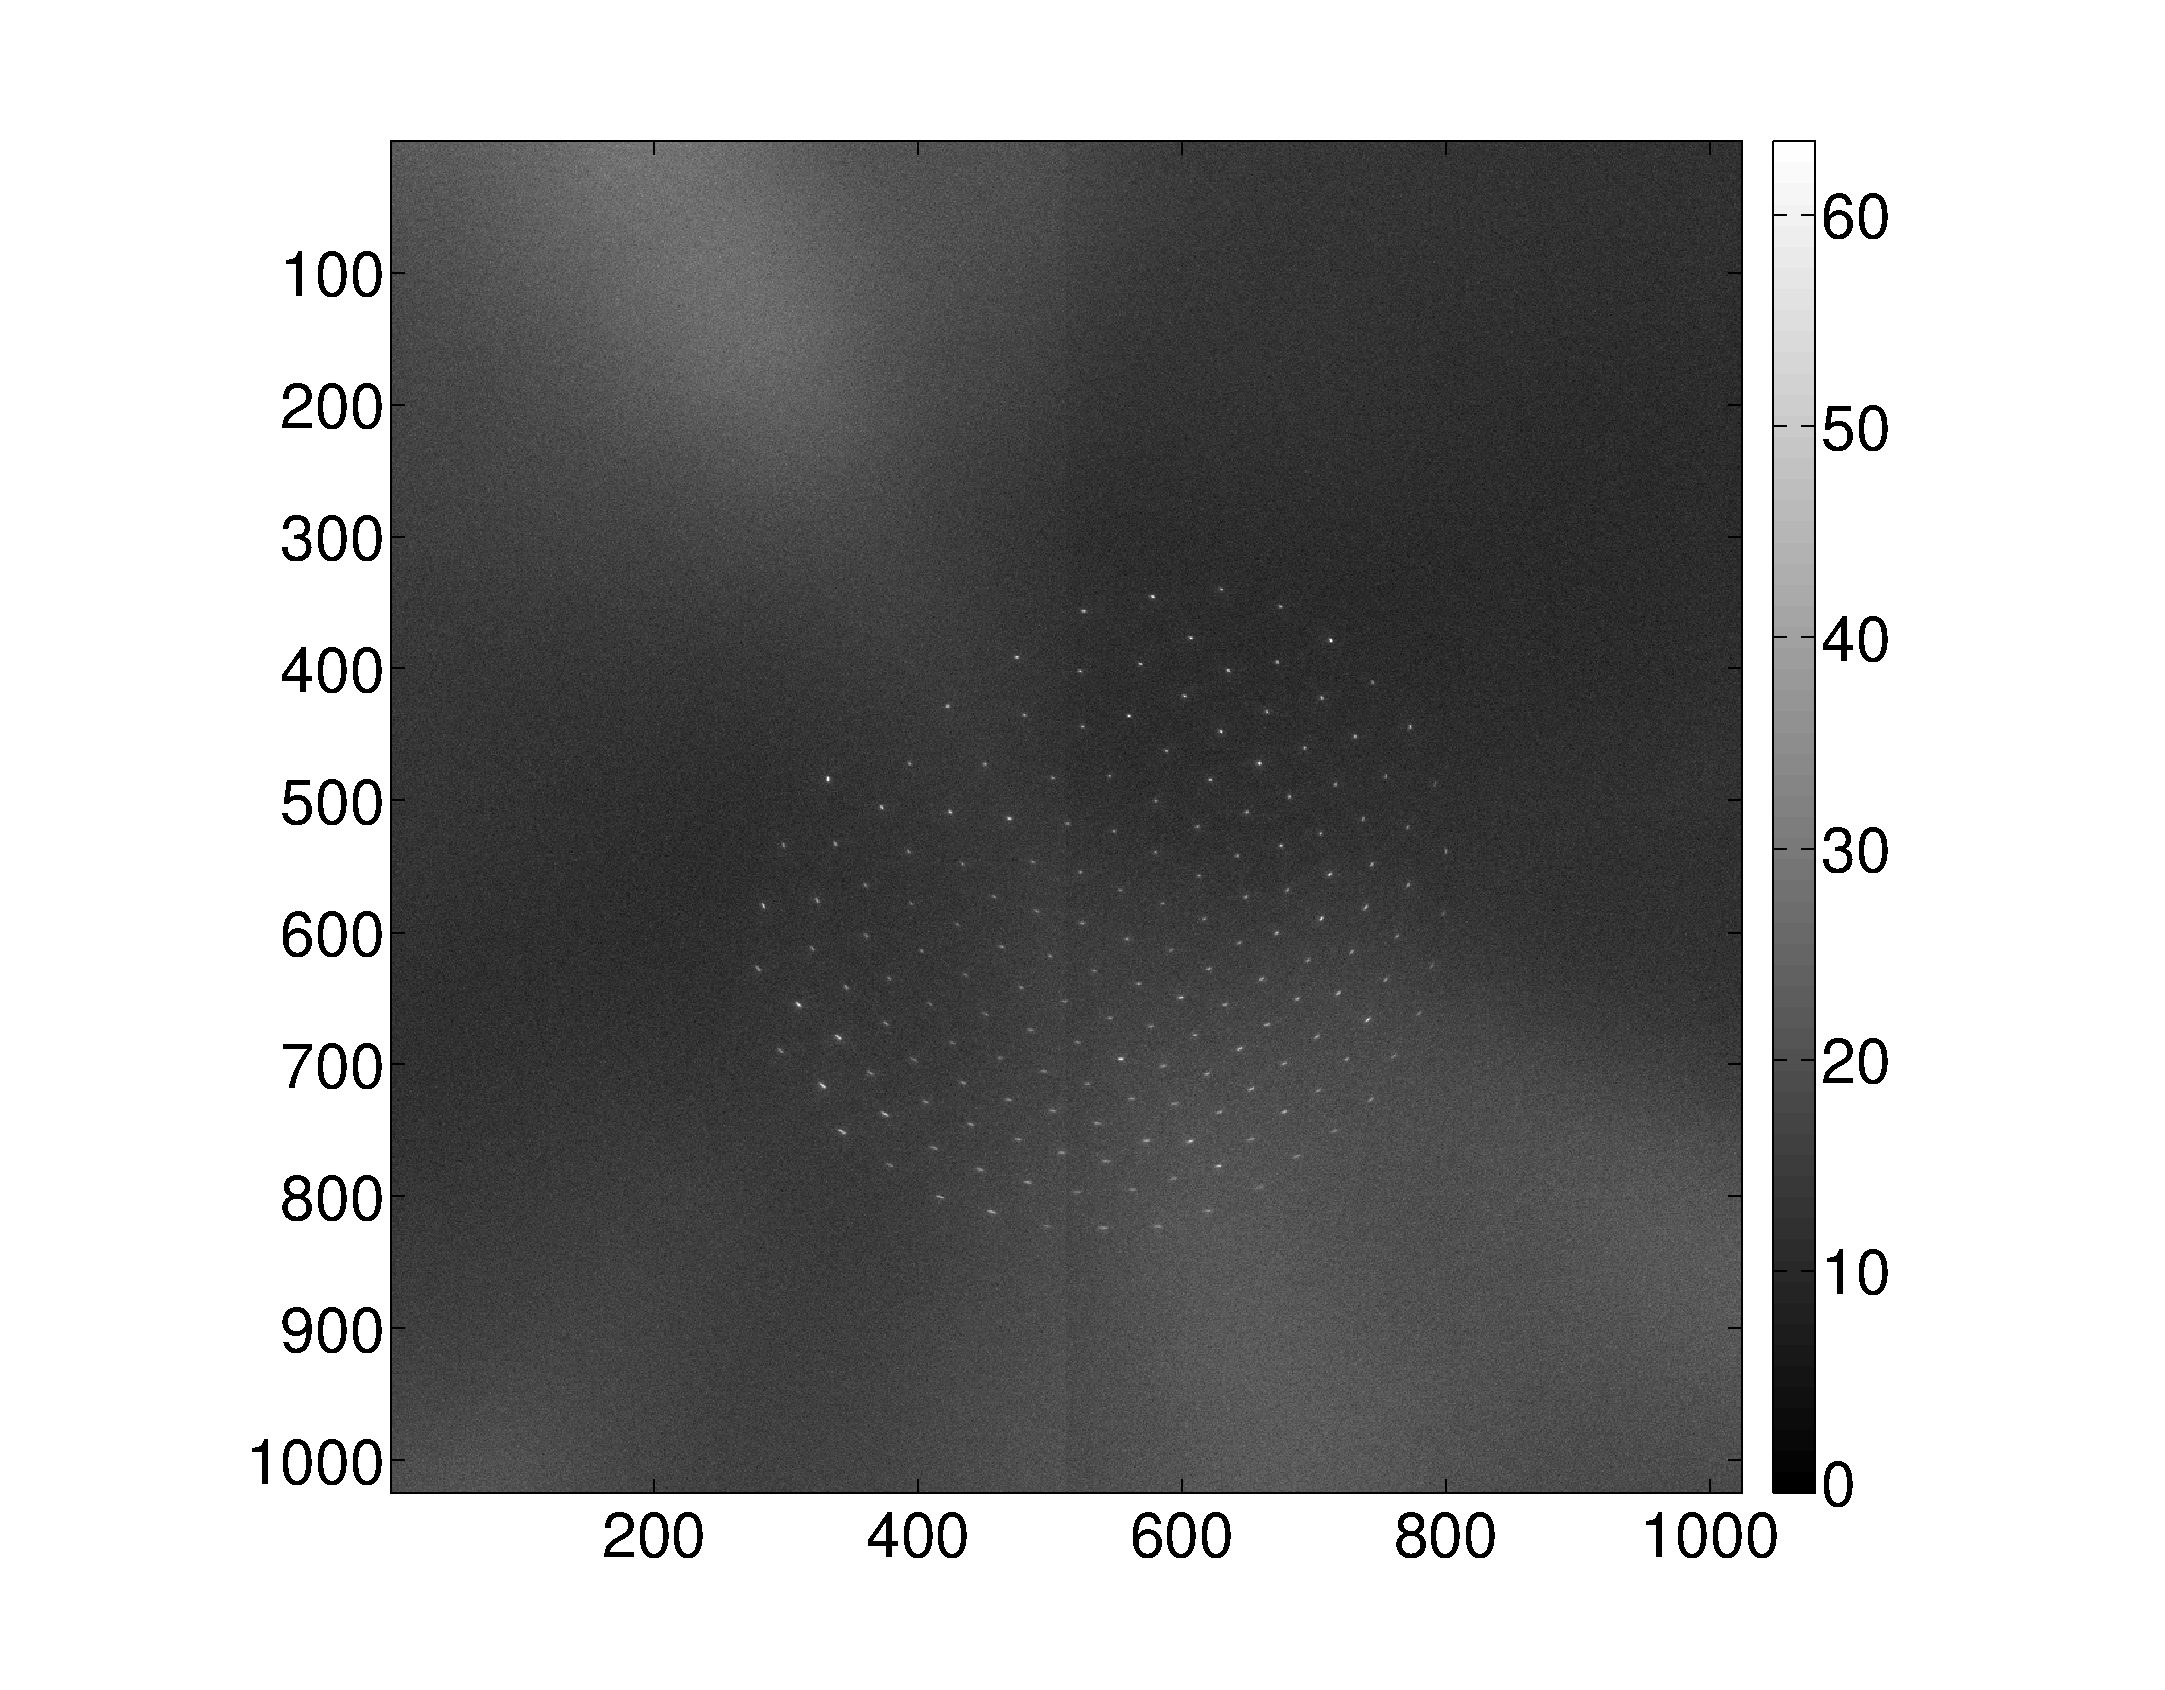
\includegraphics[width=0.95\columnwidth]{figures/eps/000000606627.eps}%
			\label{fig:forgo}
		}
		\caption{Két különböző kísérlet során készült fénykép.}
		\label{fig:captures}
	\end{figure}
	
	A fényképek alapján a részecskék pozíciójára és időbeli {\color{red}mozgására} vagyunk kíváncsiak.
	A kamera objektíve által leképezett kép a függőleges irányú pozíciót nem tartalmazza. Mivel jelen
	kísérletek során az ezirányú mozgása a részecskéknek nem számottevő, így az $x-y$ pozícióját jól
	lehet számítani a kép alapján. Nagy pontosság esetén szükséges a képek előzetes feldolgozása a
	perspektivikus torzítás kiküszöbölése végett. Természetesen ez lehetséges a pozíciók számítása után
	is, aminek a számításigénye kissebb is.
	\todo{mi kerül kimentésre}
	



